% (find-LATEX "2022-2-C2-somas-de-riemann.tex")
% (defun c () (interactive) (find-LATEXsh "lualatex -record 2022-2-C2-somas-de-riemann.tex" :end))
% (defun C () (interactive) (find-LATEXsh "lualatex 2022-2-C2-somas-de-riemann.tex" "Success!!!"))
% (defun D () (interactive) (find-pdf-page      "~/LATEX/2022-2-C2-somas-de-riemann.pdf"))
% (defun d () (interactive) (find-pdftools-page "~/LATEX/2022-2-C2-somas-de-riemann.pdf"))
% (defun e () (interactive) (find-LATEX "2022-2-C2-somas-de-riemann.tex"))
% (defun o () (interactive) (find-LATEX "2022-2-C2-somas-de-riemann.tex"))
% (defun u () (interactive) (find-latex-upload-links "2022-2-C2-somas-de-riemann"))
% (defun v () (interactive) (find-2a '(e) '(d)))
% (defun d0 () (interactive) (find-ebuffer "2022-2-C2-somas-de-riemann.pdf"))
% (defun cv () (interactive) (C) (ee-kill-this-buffer) (v) (g))
%          (code-eec-LATEX "2022-2-C2-somas-de-riemann")
% (find-pdf-page   "~/LATEX/2022-2-C2-somas-de-riemann.pdf")
% (find-sh0 "cp -v  ~/LATEX/2022-2-C2-somas-de-riemann.pdf /tmp/")
% (find-sh0 "cp -v  ~/LATEX/2022-2-C2-somas-de-riemann.pdf /tmp/pen/")
%     (find-xournalpp "/tmp/2022-2-C2-somas-de-riemann.pdf")
%   file:///home/edrx/LATEX/2022-2-C2-somas-de-riemann.pdf
%               file:///tmp/2022-2-C2-somas-de-riemann.pdf
%           file:///tmp/pen/2022-2-C2-somas-de-riemann.pdf
% http://angg.twu.net/LATEX/2022-2-C2-somas-de-riemann.pdf
% (find-LATEX "2019.mk")
% (find-sh0 "cd ~/LUA/; cp -v Pict2e1.lua Pict2e1-1.lua Piecewise1.lua ~/LATEX/")
% (find-sh0 "cd ~/LUA/; cp -v Pict2e1.lua Pict2e1-1.lua Pict3D1.lua ~/LATEX/")
% (find-sh0 "cd ~/LUA/; cp -v C2Subst1.lua C2Formulas1.lua ~/LATEX/")
% (find-CN-aula-links "2022-2-C2-somas-de-riemann" "2" "c2m222sr" "c2sr")

% «.defs»			(to "defs")
% «.title»			(to "title")
% «.links»			(to "links")
% «.somas-de-riemann-0»		(to "somas-de-riemann-0")
% «.atirei»			(to "atirei")
% «.somas-de-retangulos»	(to "somas-de-retangulos")
% «.exercicio-1»		(to "exercicio-1")
% «.somatorios»			(to "somatorios")
% «.exercicio-2»		(to "exercicio-2")
% «.jeito-esperto»		(to "jeito-esperto")
% «.exercicio-3»		(to "exercicio-3")
% «.exercicio-4»		(to "exercicio-4")
% «.mountains»			(to "mountains")
% «.soma-superior-e»		(to "soma-superior-e")
% «.set-comprehensions»		(to "set-comprehensions")
% «.lua-and-haskell»		(to "lua-and-haskell")
% «.imagens-de-finitos»		(to "imagens-de-finitos")
% «.imagens-de-conjuntos»	(to "imagens-de-conjuntos")
% «.imagens-de-intervalos»	(to "imagens-de-intervalos")
% «.exercicio-7»		(to "exercicio-7")
% «.acima-e-abaixo»		(to "acima-e-abaixo")
% «.para-todo-e-existe»		(to "para-todo-e-existe")
% «.visualizando-fas-e-exs»	(to "visualizando-fas-e-exs")
% «.visualizando-fas-e-exs-2»	(to "visualizando-fas-e-exs-2")
% «.instrucoes-des-defs»	(to "instrucoes-des-defs")
% «.instrucoes-des-1»		(to "instrucoes-des-1")
% «.instrucoes-des-2»		(to "instrucoes-des-2")
% «.exercicio-8»		(to "exercicio-8")
% «.exercicio-8-figs»		(to "exercicio-8-figs")
% «.exercicio-9»		(to "exercicio-9")
% «.na-semana-academica»	(to "na-semana-academica")
% «.quantificadores»		(to "quantificadores")
% «.elemento-neutro»		(to "elemento-neutro")
% «.vis-props»			(to "vis-props")
%
% «.djvuize»			(to "djvuize")



% <videos>
% Video (not yet):
% (find-ssr-links     "c2m222sr" "2022-2-C2-somas-de-riemann")
% (code-eevvideo      "c2m222sr" "2022-2-C2-somas-de-riemann")
% (code-eevlinksvideo "c2m222sr" "2022-2-C2-somas-de-riemann")
% (find-c2m222srvideo "0:00")

\documentclass[oneside,12pt]{article}
\usepackage[colorlinks,citecolor=DarkRed,urlcolor=DarkRed]{hyperref} % (find-es "tex" "hyperref")
\usepackage{amsmath}
\usepackage{amsfonts}
\usepackage{amssymb}
\usepackage{pict2e}
\usepackage[x11names,svgnames]{xcolor} % (find-es "tex" "xcolor")
\usepackage{colorweb}                  % (find-es "tex" "colorweb")
%\usepackage{tikz}
%
% (find-dn6 "preamble6.lua" "preamble0")
%\usepackage{proof}   % For derivation trees ("%:" lines)
%\input diagxy        % For 2D diagrams ("%D" lines)
%\xyoption{curve}     % For the ".curve=" feature in 2D diagrams
%
\usepackage{edrx21}               % (find-LATEX "edrx21.sty")
\input edrxaccents.tex            % (find-LATEX "edrxaccents.tex")
\input edrx21chars.tex            % (find-LATEX "edrx21chars.tex")
\input edrxheadfoot.tex           % (find-LATEX "edrxheadfoot.tex")
\input edrxgac2.tex               % (find-LATEX "edrxgac2.tex")
%\usepackage{emaxima}              % (find-LATEX "emaxima.sty")
%
%\usepackage[backend=biber,
%   style=alphabetic]{biblatex}            % (find-es "tex" "biber")
%\addbibresource{catsem-slides.bib}        % (find-LATEX "catsem-slides.bib")
%
% (find-es "tex" "geometry")
\usepackage[a6paper, landscape,
            top=1.5cm, bottom=.25cm, left=1cm, right=1cm, includefoot
           ]{geometry}
%
\begin{document}

\catcode`\^^J=10
\directlua{dofile "dednat6load.lua"}  % (find-LATEX "dednat6load.lua")
%L dofile "Piecewise1.lua"           -- (find-LATEX "Piecewise1.lua")
%L dofile "QVis1.lua"                -- (find-LATEX "QVis1.lua")
%L dofile "Pict3D1.lua"              -- (find-LATEX "Pict3D1.lua")
%L dofile "C2Formulas1.lua"          -- (find-LATEX "C2Formulas1.lua")
%L Pict2e.__index.suffix = "%"
\pu
\def\pictgridstyle{\color{GrayPale}\linethickness{0.3pt}}
\def\pictaxesstyle{\linethickness{0.5pt}}
\def\pictnaxesstyle{\color{GrayPale}\linethickness{0.5pt}}
\celllower=2.5pt

% «defs»  (to ".defs")
% (find-LATEX "edrx21defs.tex" "colors")
% (find-LATEX "edrx21.sty")

\def\u#1{\par{\footnotesize \url{#1}}}

\def\drafturl{http://angg.twu.net/LATEX/2022-2-C2.pdf}
\def\drafturl{http://angg.twu.net/2022.2-C2.html}
\def\draftfooter{\tiny \href{\drafturl}{\jobname{}} \ColorBrown{\shorttoday{} \hours}}

\def\V{\mathbf{V}}
\def\F{\mathbf{F}}

% https://en.wikipedia.org/wiki/Extended_real_number_line
\def\Rext{\overline{\R}}


%  _____ _ _   _                               
% |_   _(_) |_| | ___   _ __   __ _  __ _  ___ 
%   | | | | __| |/ _ \ | '_ \ / _` |/ _` |/ _ \
%   | | | | |_| |  __/ | |_) | (_| | (_| |  __/
%   |_| |_|\__|_|\___| | .__/ \__,_|\__, |\___|
%                      |_|          |___/      
%
% «title»  (to ".title")
% (c2m222srp 1 "title")
% (c2m222sra   "title")

\thispagestyle{empty}

\begin{center}

\vspace*{1.2cm}

{\bf \Large Cálculo 2 - 2022.2}

\bsk

Aula 13, 14 e 16: Somas de Riemann,

imagens de conjuntos, e infs e sups

\bsk

Eduardo Ochs - RCN/PURO/UFF

\url{http://angg.twu.net/2022.2-C2.html}

\end{center}

\newpage

% «links»  (to ".links")
% (c2m222srp 2 "links")
% (c2m222sra   "links")
% (c2m221tfc1a "title")
% (c2m221tfc1a "title" "Aula 23: o TFC1")
% (c2m221isa "title")
% (c2m221isa "title" "Aula 15: infs e sups")
% (find-THfile "2022-apresentacao-sobre-C2.blogme" "tudos.txt")
% (c2m221tudop 1 "title")
% (c2m221tudoa   "title")
% (c2m212tudop 1 "title")
% (c2m212tudoa   "title")
% (find-pdf-text   "~/LATEX/2022-1-C2-tudo.pdf")
% (find-pdf-text   "~/LATEX/2021-2-C2-tudo.pdf")
% (find-pdf-text   "~/LATEX/2021-1-C2-tudo.pdf")
% (find-pdf-text   "~/LATEX/2020-2-C2-tudo.pdf")


\newpage

% «somas-de-riemann-0»  (to ".somas-de-riemann-0")
% (c2m222srp 2 "somas-de-riemann-0")
% (c2m222sra   "somas-de-riemann-0")

{\bf Introdução: Somas de Riemann}

\scalebox{0.55}{\def\colwidth{10cm}\firstcol{

Somas de Riemann podem ser definidas de vários jeitos diferentes. A
figura abaixo tem dois desses jeitos: os retângulos mais escuros dela
são a ``\ColorRed{melhor aproximação por retângulos por baixo}'' para
$\Intx{-1}{1}{f(x)}$; repare que todos esses retângulos mais escuros
estão ``apoiados no eixo $x$''...

% (find-c2crishernandezpage (+ 10  2) "")
% (find-latexgimp-links "2020-1-C2/area-hernandez-1")

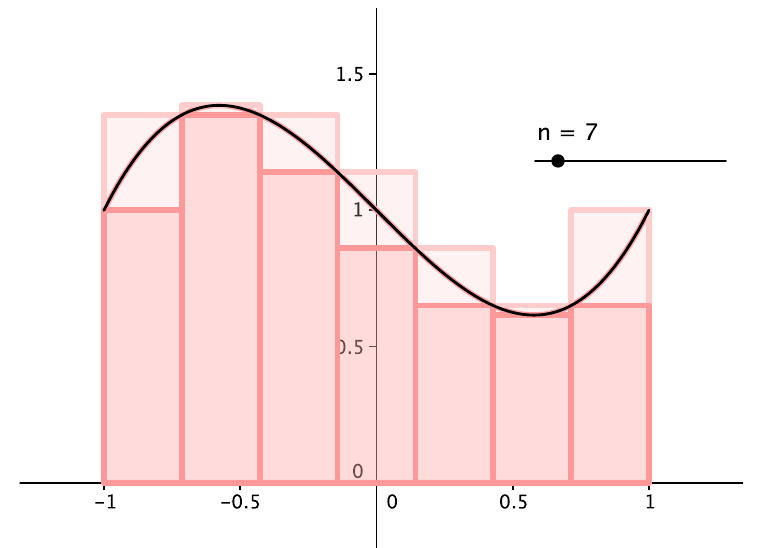
\includegraphics[width=8cm]{2020-1-C2/area-hernandez-1.png}

Nós vamos considerar que os retângulos mais claros da figura também
estão apoiados no eixo $x$, só que eles estão atrás dos mais escuros,
então a gente só vê uma parte deles.

\msk

Esses retângulos mais claros -- que, deixa eu repetir, estão todos
apoiados no eixo $x$ -- são a ``\ColorRed{melhor aproximação por
  retângulos por cima}'' para $\Intx{-1}{1}{f(x)}$.

}\anothercol{

Dá pra fazer uma figura como essas na mão e no olhômetro assim: 1) a
gente começa desenhando uma curva $y=f(x)$; 2) depois a gente desenha
a parede esquerda da região $\Intx{a}{b}{f(x)}$, que é um segmento
vertical em $x=a$, e a parede direita, que é um segmento em $x=b$; 3)
depois a gente divide o intervalo de integração, $[a,b]$, em um certo
número de subintervalos -- a Cristiane Hernández usou o intervalo
$[-1,1]$ e dividiu ele em 7 subintervalos iguais; 4) pra cada um
desses subintervalos a gente desenha o retângulo mais alto cuja base é
aquele intervalo e que está todo sob a curva $y=f(x)$; 5) pra cada um
desses subintervalos a gente desenha o retângulo mais baixo cuja base
é aquele intervalo e que está todo acima da curva $y=f(x)$; 6) aí a
gente colore tudo do jeito certo, usando uma cor pra ``melhor
aproximação por retângulos por baixo'' -- os retângulos do passo 4 --
e outra cor pra ``melhor aproximação por retângulos por cim'' -- os
retângulos do passo 5.

\msk

Eu peguei a figura à esquerda das notas da Cristiane Hernández. Link:

{\scriptsize

% (c2sop 4 "fig-hernandez-1")
% (c2soa   "fig-hernandez-1")
% (find-books "__analysis/__analysis.el" "hernandez")
% (find-hernandezpage (+ 10   2)   "As Figuras de 2 a 5")
% (find-hernandeztext (+ 10   2)   "As Figuras de 2 a 5")
%    http://angg.twu.net/2015.1-C2/CALCULOIIA_EAD_Versao_Final_correcao_aulas_25_a_30.pdf#page=12
\url{http://angg.twu.net/2015.1-C2/CALCULOIIA_EAD_Versao_Final_correcao_aulas_25_a_30.pdf\#page=12}

}

}}

\newpage

%     _   _   _          _ 
%    / \ | |_(_)_ __ ___(_)
%   / _ \| __| | '__/ _ \ |
%  / ___ \ |_| | | |  __/ |
% /_/   \_\__|_|_|  \___|_|
%                          
% «atirei»  (to ".atirei")
% (c2m222srp 3 "atirei")
% (c2m222sra   "atirei")
% (c2m212mt2p 6 "atirei-o-pau-no-gato")
% (c2m212mt2a   "atirei-o-pau-no-gato")

{\bf Atirei o Pau no Gato: seja como o Bob}

\scalebox{0.77}{\def\colwidth{7.2cm}\firstcol{

Imagina que você está fazendo aula de flauta doce junto com o Alex e o
Bob, e na prova vocês vão ter que tocar Atirei o Pau no Gato.

O Alex demora um tempão pra encontrar cada nota, e ele leva meia hora
pra tocar a música toda.

O Bob toca a música toda certinha em menos de 30 segundos.

Quando saem as notas o Alex tirou uma nota baixa e o Bob tirou 10.

Aí o Alex vai chorar pontos e diz ``{\sl pôxa, profe, eu me esforcei
  muito!}''

\bsk

Quando o Bob tocou Atirei o Pau no Gato ele fez a música {\sl parecer
  fácil}. O esforço dele {\sl ficou invisível}.

\msk

\standout{Seja como o Bob.}

%\bsk
%\bsk


}\anothercol{

O que a gente vai fazer neste PDF vai parecer com o Atirei o Pau no
Gato, só que com somatórios e retângulos e trapézios ao invés de
notas. Você vai aprender a visualizar e a desenhar figuras com dezenas
de retângulos e trapézios {\sl em poucos segundos} -- e você quer
chegar no ponto em que fazer esses desenhos passa a ser bem fácil.

}}


\newpage

% «somas-de-retangulos»  (to ".somas-de-retangulos")
% (c2m222srp 4 "somas-de-retangulos")
% (c2m222sra   "somas-de-retangulos")

{\bf Somas de retângulos}

\scalebox{0.5}{\def\colwidth{10.5cm}\firstcol{

No ``item 5'' da aula sobre o Mathologermóvel -- links:

\ssk

{\footnotesize

% (c2m222mmp 5 "item-5")
% (c2m222mma   "item-5")
%    http://angg.twu.net/LATEX/2022-2-C2-mathologermovel.pdf#page=5
\url{http://angg.twu.net/LATEX/2022-2-C2-mathologermovel.pdf\#page=5}

% (c2m221tfc1p 7 "exercicio-1")
% (c2m221tfc1a   "exercicio-1")
%    http://angg.twu.net/LATEX/2022-1-C2-TFC1.pdf#page=7
\url{http://angg.twu.net/LATEX/2022-1-C2-TFC1.pdf\#page=7}

}

\ssk

você aprendeu a calcular áreas de figuras ``feitas de retângulos'', e
como essas áreas representavam {\sl distâncias} você sabia que algumas
áreas iriam ``contar negativamente''...

Agora a gente vai fazer o contrário do que a gente fez naquela aula.
Ao invés da gente transformar uma figura feita de retângulos -- cuja
área a gente quer calcular -- numa expressão como esta aqui,
%
$$2(2-1.5)+3(4-2)$$
%
a gente vai transformar expressões como essa acima numa figura feita
de retângulos. A convenção vai ser essa aqui. Por exemplo, em
%
$$3(4-2)
$$
%
o 3 vai ser a altura do retângulo e $(4-2)$ vai ser a base dele. Mais
precisamente, o ``3'' diz que o teto desse retângulo vai estar em
$y=3$, e o ``$(4-2)$'' diz que a base dele vai de $x=2$ até $x=4$, e
como nós agora só estamos interessados em retângulos apoiados no eixo
$x$ o chão dele vai ter $y=0$. Ou seja, os vértices dele vão ser:
%
$$\begin{array}{cc}
  (2,3), & (4,3), \\
  (2,0), & (4,0). \\
  \end{array}
$$

}\anothercol{

Lembre que matemáticos e físicos pensam de jeitos muito diferentes.
Por exemplo, é comum livros de Física dizerem coisas tipo ``áreas
negativas não existem, então temos que fazer o ajuste tal'', ou ``a
massa não pode ser negativa, então blá'', e é comum livros de
Matemática dizerem coisas tipo ``vamos supor que existe um número $i$
tal que $i^2=-1$. Então esse número $i$ vai ter que ter as
propriedades tais e tais...''

Lembre também que na aula de 29/setembro eu fiz uma figura sobre
generalizar e depois disso obter outros casos particulares da fórmula
geral... dá pra acessar essa figura aqui:

\ssk

{\footnotesize

% (find-angg ".emacs" "c2q222" "set29:")
% (find-c2q222page 24 "set29: substituição trigonométrica (2)")
%    http://angg.twu.net/2022.2-C2/C2-quadros.pdf#page=24
\url{http://angg.twu.net/2022.2-C2/C2-quadros.pdf\#page=24}

}

Aqui nós vamos pensar ``como matemáticos'', e pra gente isso aqui
%
$$y·(x_d-x_e)$$
%
``vai ser'' um retângulo apoiado no eixo $x$, com altura $y$ e base
indo de $x_e$ (``extremidade esquerda'') até $x_d$ (``extremidade
direita'')... a representação gráfica dele vai ser a que eu descrevi
acima, e a área dele vai ser o resultado numérico de $y·(x_d-x_e)$ --
que pode dar um número negativo!...

}}



\newpage

% «exercicio-1»  (to ".exercicio-1")
% (c2m222srp 5 "exercicio-1")
% (c2m222sra   "exercicio-1")

{\bf Exercício 1}

\scalebox{0.9}{\def\colwidth{12cm}\firstcol{

a) Verifique que $3(4-2)$ e $3(2-4)$ são dois retângulos que têm a
mesma interpretação geométrica, mas um tem área positiva e o outro tem
área negativa.

\msk

Depois leia as páginas 35 e 36 daqui,

\ssk

{\scriptsize

% (c2m211prp 35 "retangulos-degenerados")
% (c2m211pra    "retangulos-degenerados")
%    http://angg.twu.net/LATEX/2021-1-C2-propriedades-da-integral.pdf#page=35
\url{http://angg.twu.net/LATEX/2021-1-C2-propriedades-da-integral.pdf\#page=35}

}

\ssk

e os dois links da página 35 pra Wikipedia em português, e represente
graficamente cada um dos retângulos abaixo:

\msk

b) $(-3)(2-4)$

c) $(-3)(4-2)$

d) $0(4-2)$

e) $0(2-2)$

f) $3(2-2)$

\msk

Pra nós todos eles são ``retângulos''. Na definição da Wikipedia quais
deles são ``retângulos degenerados''?

}\anothercol{
}}

\newpage

%  ____                        _             _           
% / ___|  ___  _ __ ___   __ _| |_ ___  _ __(_) ___  ___ 
% \___ \ / _ \| '_ ` _ \ / _` | __/ _ \| '__| |/ _ \/ __|
%  ___) | (_) | | | | | | (_| | || (_) | |  | | (_) \__ \
% |____/ \___/|_| |_| |_|\__,_|\__\___/|_|  |_|\___/|___/
%                                                        
% «somatorios»  (to ".somatorios")
% (c2m222srp 6 "somatorios")
% (c2m222sra   "somatorios")

{\bf Somatórios}

Dá pra expandir somatórios tanto em um passo só

como em dois passos, como aqui:
%
$$\scalebox{0.9}{$
  \begin{array}{rcl}
    \sum_{k=2}^{5} 10^k &=& 10^2 + 10^3 + 10^4 + 10^5 \\[5pt]
    \sum_{k=2}^{5} 10^k &=& (10^k) [k:=2] \\
                        &+& (10^k) [k:=3] \\
                        &+& (10^k) [k:=4] \\
                        &+& (10^k) [k:=5] \\[2.5pt]
                        &=& 10^2 + 10^3 + 10^4 + 10^5 \\
  \end{array}
  $}
$$

% «exercicio-2»  (to ".exercicio-2")
% (c2m222srp 6 "exercicio-2")
% (c2m222sra   "exercicio-2")

{\bf Exercício 2}

Veja esta página aqui para os detalhes,

%\ssk

{\footnotesize

% (c2m212introp 13 "somatorios")
% (c2m212introa    "somatorios")
%    http://angg.twu.net/LATEX/2021-2-C2-intro.pdf#page=13
\url{http://angg.twu.net/LATEX/2021-2-C2-intro.pdf#page=13}

}

%\ssk

e faça todos os itens do Exercício 3 dela.

\newpage

%      _      _ _                                    _        
%     | | ___(_) |_ ___     ___  ___ _ __   ___ _ __| |_ ___  
%  _  | |/ _ \ | __/ _ \   / _ \/ __| '_ \ / _ \ '__| __/ _ \ 
% | |_| |  __/ | || (_) | |  __/\__ \ |_) |  __/ |  | || (_) |
%  \___/ \___|_|\__\___/   \___||___/ .__/ \___|_|   \__\___/ 
%                                   |_|                       
% «jeito-esperto»  (to ".jeito-esperto")
% (c2m222srp 7 "jeito-esperto")
% (c2m222sra   "jeito-esperto")

{\bf O jeito esperto}

\ssk

Leia as páginas 6 e 7 daqui:

{\footnotesize

% (c2m211somas1p 6 "exercicio-1")
% (c2m211somas1a   "exercicio-1")
% (c2m212somas1p 7 "jeito-esperto")
% (c2m212somas1a   "jeito-esperto")
%    http://angg.twu.net/LATEX/2021-2-C2-somas-1.pdf#page=7
\url{http://angg.twu.net/LATEX/2021-2-C2-somas-1.pdf#page=7}

}

\bsk

% «exercicio-3»  (to ".exercicio-3")
% (c2m222srp 7 "exercicio-3")
% (c2m222sra   "exercicio-3")

{\bf Exercício 3}

\ssk

a) Faça o exercício 1 da página 6 desse PDF --

o que pede pra você desenhar uma parábola.

\ssk

b) Desenhe sobre essa parábola o retângulo $f(0.5)(1-0.5)$.

Aqui você \standout{TEM} que usar o ``jeito esperto''.

\bsk

Se você não aprender a usar o jeito esperto:

$•$ você vai demorar muito,

$•$ seu retângulo não vai ter um vértice sobre a parábola,

$•$ e você nunca vai virar o Bob.

\newpage

% «exercicio-4»  (to ".exercicio-4")
% (c2m222srp 8 "exercicio-4")
% (c2m222sra   "exercicio-4")
% (c2m221somas3p 4 "exercicio-1")
% (c2m221somas3a   "exercicio-1")

{\bf Exercício 4.}

\def\sumo{\sum_{i=1}^{8}}
\def\sumoo#1{\sumo #1 (x_i - x_{i-1})}

\scalebox{0.9}{\def\colwidth{12cm}\firstcol{

Seja $f(x)$ a função da próxima página.

Você vai receber (pelo menos) uma cópia dessa página.

Faça cada item abaixo em um dos 12 gráficos da $f(x)$.

\msk

Represente graficamente cada um dos somatórios abaixo.

Se você tiver dificuldade com algum desses somatórios

comece expandindo ele em dois passos, como na página 7.

\msk

a) $\sumoo{f(x_i)}$

\ssk

b) $\sumoo{f(x_{i-1})}$

\ssk

c) $\sumoo{\max(f(x_{i-1}), f(x_i))}$

\ssk

d) $\sumoo{\min(f(x_{i-1}), f(x_i))}$

\ssk

e) $\sumoo{f(\frac{x_{i-1} + x_i}{2})}$

\ssk

f) $\sumoo{\frac{f(x_{i-1}) + f(x_i)}{2}}$

}\anothercol{
}}


\newpage


%  __  __                   _        _           
% |  \/  | ___  _   _ _ __ | |_ __ _(_)_ __  ___ 
% | |\/| |/ _ \| | | | '_ \| __/ _` | | '_ \/ __|
% | |  | | (_) | |_| | | | | || (_| | | | | \__ \
% |_|  |_|\___/ \__,_|_| |_|\__\__,_|_|_| |_|___/
%                                                
% «mountains»  (to ".mountains")
% (c2m222srp 9 "mountains")
% (c2m222sra   "mountains")
% (c2m221somas3p 3 "mountains")
% (c2m221somas3a   "mountains")

% (find-angg "LUA/Piecewise1.lua" "Xtoxytoy-test2")
%
%L Pict2e.bounds = PictBounds.new(v(0,0), v(23,9))
%L spec   = "(0,1)--(5,6)--(7,4)--(11,8)--(15,4)--(17,6)--(23,0)"
%L xs     = {    1,3,    6,     9,  11, 13,   16,19,    21      }
%L labely = -1
%L pws    = PwSpec.from(spec)
%L xtos   = Xtoxytoy.from(pws:fun(), xs)
%L vlines = xtos:topict("v")
%L curve  = pws:topict()
%L labels = PictList {}
%L for i,x in ipairs(xs) do
%L   labels:addputstrat(v(x,labely), "\\cell{x_"..(i-1).."}")
%L end
%L p = PictList { vlines, curve:prethickness("2pt"), labels }
%L p:pgat("pA", "mountain"):output()
\pu

\unitlength=8pt

\vspace*{-0.25cm}
\hspace*{-0.5cm}
$\scalebox{0.55}{$
 \begin{array}{ccccc}
 \mountain && \mountain && \mountain \\[20pt]
 \mountain && \mountain && \mountain \\[20pt]
 \mountain && \mountain && \mountain \\[20pt]
 \mountain && \mountain && \mountain \\[20pt]
 \end{array}
 $}
$

\newpage

%            _                                               
%  _ __ ___ (_)_ __          ___   _ __ ___   __ ___  __     
% | '_ ` _ \| | '_ \        / _ \ | '_ ` _ \ / _` \ \/ /     
% | | | | | | | | | |      |  __/ | | | | | | (_| |>  <      
% |_| |_| |_|_|_| |_|____   \___| |_| |_| |_|\__,_/_/\_\____ 
%                  |_____|                            |_____|
%
% «soma-superior-e»  (to ".soma-superior-e")
% (c2m222srp 10 "soma-superior-e")
% (c2m222sra    "soma-superior-e")

{\bf Soma superior e soma inferior}

\scalebox{0.7}{\def\colwidth{12cm}\firstcol{

Nas páginas 217 e 218 o Miranda define as notações
%
$$\min_{x∈I} f(x)
  \qquad
  \text{e}
  \qquad
  \max_{x∈I} f(x)
$$

usando o truque do ``vire-se'': ele mostra uma figura e o

leitor tem que se virar pra entender o que essas notações

querem dizer... veja:

\ssk

{\scriptsize

% (find-books "__analysis/__analysis.el" "miranda")
% (find-books "__analysis/__analysis.el" "miranda" "soma superior")
% (find-dmirandacalcpage 217   "soma superior e inferior")
% (find-dmirandacalcpage 218   "min_")
%    http://hostel.ufabc.edu.br/~daniel.miranda/calculo/calculo.pdf#page=218
\url{http://hostel.ufabc.edu.br/~daniel.miranda/calculo/calculo.pdf\#page=218}

}

\msk

{\bf Exercício 5.}

a) Entenda o que essas notações do Miranda querem dizer

e verifique que nas figuras da página 9 temos:
%
$$\begin{array}{ccccc}
   && \D \max(f(x_1),f(x_2))
     &\lneqq& \D \max_{x∈[x_1,x_2]}f(x) \\
   \D     \min_{x∈[x_2,x_3]}f(x)
     &\lneqq& \min(f(x_2),f(x_3)) \\
  \end{array}
$$

e depois represente nos gráficos da página 9:

\ssk

b) $\sumoo{(\max_{x∈[x_{i-1},x_i]} f(x))}$

\ssk

c) $\sumoo{(\min_{x∈[x_{i-1},x_i]} f(x))}$


}\anothercol{
}}

\newpage

% «set-comprehensions»  (to ".set-comprehensions")
% (c2m222srp 99 "set-comprehensions")
% (c2m222sra    "set-comprehensions")

{\bf ``Set comprehensions''}


\scalebox{0.55}{\def\colwidth{13cm}\firstcol{

Lembre que:
%
$$\begin{array}{rcl}
  \setofst{ a∈\{1,2,3,4\} }{ a≥3 } &=& \{3,4\}, \\
  \setofst{ 10a }{ a∈\{1,2,3,4\} } &=& \{10,20,30,40\}... \\
  \end{array}
$$

Se você não lembrar tente ler as páginas 8 a 12 daqui,

\ssk

{\scriptsize

% (mpgp 8 "comprehension")
% (mpga   "comprehension")
%    http://angg.twu.net/LATEX/material-para-GA.pdf#page=8
\url{http://angg.twu.net/LATEX/material-para-GA.pdf\#page=8}

}

\ssk

que tem explicações e exercícios, mas as explicações estão escritas
numa ordem estranha... $\frown$

\msk

Resumindo muitíssimo: existem dois tipos diferentes de notações da
forma ``$\setofst{\ldots}{\ldots}$'', e um bom modo de entender como
elas funcionam é anotar quais pedaços delas são ``geradores'', quais
são ``filtros'', e quais são ``resultado''; os ``geradores''
funcionam como o `for' de uma linguagem de programação, os filtros
funcionam como um `if' -- ou, mais precisamente, como um ``if not ...
then break'' -- e o ``resultado'' funciona como um `print'.

\bsk

{\bf Exercício 6.}

Entenda a expressão abaixo e calcule o resultado dela:
%
\def\undt#1#2{\underbrace{#1}_{\text{#2}}}
\def\uger #1{\undt{#1}{gerador}}
\def\ufilt#1{\undt{#1}{filtro}}
\def\ures #1{\undt{#1}{resultado}}
%
$$\setofst{\ures{(x,y)}}{
           \uger{y∈\{0,1,2,3\}},
           \uger{x∈\{0,\ldots,y\}},
           \ufilt{x+y≤5}
          }
$$

e compare-a com estes programinhas em Lua e Haskell:

\ssk

{\scriptsize

%                 (xz "~/2022.2-C2/set_comprehensions_in_lua_and_haskell.png")
%         (find-fline "~/2022.2-C2/set_comprehensions_in_lua_and_haskell.png")
%    http://angg.twu.net/2022.2-C2/set_comprehensions_in_lua_and_haskell.png
\url{http://angg.twu.net/2022.2-C2/set_comprehensions_in_lua_and_haskell.png}

}

}\anothercol{
}}

% «lua-and-haskell»  (to ".lua-and-haskell")
% (c2m222srp 8 "lua-and-haskell")
% (c2m222sra   "lua-and-haskell")
% (setq eepitch-preprocess-regexp "^")
% (setq eepitch-preprocess-regexp "^%T ?")
%
%T  (eepitch-lua51)
%T  (eepitch-kill)
%T  (eepitch-lua51)
%T for y=2,0,-1 do print(y) end
%T 
%T for y=2,0,-1 do
%T   for x=0,2 do
%T     printf("(%d,%d) ", x, y)
%T   end
%T   print()
%T end
%T 
%T for y=2,0,-1 do
%T   for x=0,y do
%T     printf("(%d,%d) ", x, y)
%T   end
%T   print()
%T end
%T 
%T for y=3,0,-1 do
%T   for x=0,y do
%T     if not (x+y <= 4) then break end
%T     printf("(%d,%d) ", x, y)
%T   end
%T   print()
%T end
%T 
%T  (eepitch-ghci)
%T  (eepitch-kill)
%T  (eepitch-ghci)
%T [(x,y) | y <- [3,2..0], x <- [0..y]]
%T [(x,y) | y <- [3,2..0], x <- [0..y], x+y <= 4]



\newpage


% https://www.mathsisfun.com/sets/set-builder-notation.html
% https://en.wikipedia.org/wiki/Set-builder_notation
% (find-es "ead" "thanos-tsouanas")
% (find-books "__analysis/__analysis.el" "leithold")
% (find-books "__analysis/__analysis.el" "leithold" "intervalo aberto")
% (find-leitholdptpage (+ 17   6)   "intervalo aberto")



\newpage

% «imagens-de-finitos»  (to ".imagens-de-finitos")
% (c2m222srp 12 "imagens-de-finitos")
% (c2m222sra    "imagens-de-finitos")

{\bf Imagens de conjuntos finitos}

Veja as páginas 5 e 6 daqui:

\ssk

{\footnotesize

% (c2m221somas3p 5 "imagens-figuras")
% (c2m221somas3a   "imagens-figuras")
%    http://angg.twu.net/LATEX/2022-1-C2-somas-3.pdf#page=5
\url{http://angg.twu.net/LATEX/2022-1-C2-somas-3.pdf\#page=5}

}

\bsk
\bsk

% (find-c2q222page 30 "out06: somas de Riemann (2): dois abusos de linguagem")

Dois abusos de linguagem

(que eu expliquei no quadro):
%
$$\begin{array}{rcll}
  f(\{7,8,9\}) &=& \setofst{f(x)}{x∈\{7,8,9\}} \\
  \max(a,b,c,d,e) &=& \max(a,\max(b,\max(c,\max(d,e)))) \\
  %
  \\[-5pt]
  %
  f(\{7,8,9\}) &=& \{f(7),f(8),f(9)\},      \\
  \max(a,b,c,d,e) &=& \max(a,\max(b,c,d,e)) \\
                  &=& \max(a,\max(b,\max(c,d,e))) \\
                  &=& \max(a,\max(b,\max(c,\max(d,e)))) \\
  \end{array}
$$



\newpage

% «imagens-de-intervalos»  (to ".imagens-de-intervalos")
% (c2m222srp 13 "imagens-de-intervalos")
% (c2m222sra    "imagens-de-intervalos")

{\bf Imagens de intervalos}

\scalebox{0.5}{\def\colwidth{11.2cm}\firstcol{

Veja as páginas 5 e 7 daqui:

\ssk

{\footnotesize

% (c2m221somas3p 5 "imagens-figuras")
% (c2m221somas3a   "imagens-figuras")
%    http://angg.twu.net/LATEX/2022-1-C2-somas-3.pdf#page=5
\url{http://angg.twu.net/LATEX/2022-1-C2-somas-3.pdf\#page=5}

}

\msk

Digamos que na sua turma de Cálculo 2 tem dois Alexes diferentes, um
Bob, um Carlos e um Daniel, e todo mundo tá tentando resolver um
exercício que é o seguinte: ``seja $f$ a função da página 5 do link
acima. Calcule $f([1,3])$''.

Todo mundo reconhece que o intervalo $[1,3]$ é um conjunto com
infinitos pontos, e cada pessoa tenta resolver esse exercício de um
jeito diferente.

\msk

O Alex 1 decide começar listando todos os pontos do intervalo $[1,3]$.
Ele vai primeiro obter uma lista de pontos que ele vai escrever nesse
formato aqui,
%
$$\{x_1,x_2,x_3,x_4,\ldots\}
$$

e depois ele vai simplificar esse conjunto daqui,
%
$$\{f(x_1),f(x_2),f(x_3),f(x_4),\ldots\}
$$

transformando ele numa lista de números, pondo os números dessa lista
em ordem e deletando as repetições... \ColorRed{só que como o conjunto
  $\{x_1,x_2,x_3,x_4,\ldots\}$ é infinito ele nunca consegue terminar
  o primeiro passo.}

\msk

O Alex 2 decide que ele vai pegar uma sequência de conjuntos finitos
cada vez maiores, e ``cada vez mais parecidos'' com o conjunto
$[1,3]$. Ele escolhe essa sequência aqui...

}\anothercol{

%
$$\begin{array}{rcl}
  A_1 &=& \{1,3\}, \\
  A_2 &=& \{1,2,3\}, \\
  A_3 &=& \{1,1.5,2,2.5,3\}, \\
  A_4 &=& \{1,1.25,1.5,1.75,2,2.25,2.5,2.75,3\}, \ldots \\
  \end{array}
$$

Ele calcula $f(A_1)$, $f(A_2)$, $f(A_3)$, $f(A_4)$ pelo gráfico usando
o ``jeito esperto'' -- como nas figuras da página 5 do link -- e ele
deduz, \ColorRed{por um argumento informal e olhométrico}, que
$f([1,3])$ \ColorRed{deve ser} o intervalo $[3,4]$.

\msk

O Bob faz algo parecido como o Alex 2, mas ele encontra um modo de
``levantar'' todo o intervalo $[1,3]$ pro gráfico da função $y=f(x)$
de uma vez só, e de depois ``projetar'' pro eixo $y$ esse ``intervalo
levantado''. Ele obtém uma figura bem parecida com a última figura da
página 5 do link, e ele descobre -- \ColorRed{também meio no
  olhômetro} -- que $f([1,3]) = [3,4]$.

\msk

O Carlos vê que \ColorRed{é óbvio que}
$f([1,3]) = [f(1),f(3)] = \{3,3\} = \{3\}$, e \ColorRed{portanto} a
imagem do intervalo $[1,3]$ pela função $f$ é um conjunto com um ponto
só. $\frown$

\msk

O Daniel resolve que tudo isso é informal demais pra ele, e que ele
precisa aprender um modo 100\% preciso e formal de calcular $f([1,3])$
sem o gráfico. Ele descobre que vai ter que estudar uma coisa chamada
``Análise Matemática'', baixa o ``{\sl Elementary Analysis: The Theory
  of Calculus}'' do Kenneth Ross, começa a estudar por ele e aprende
coisa incríveis -- \ColorRed{mas ele leva um ano nisso}.

\msk

\standout{Seja como o Bob!}

}}

\newpage

% «exercicio-7»  (to ".exercicio-7")
% (c2m222srp 14 "exercicio-7")
% (c2m222sra    "exercicio-7")
% (c2m221somas3p 7 "exercicio-2")
% (c2m221somas3a   "exercicio-2")

{\bf Exercício 7.}


\scalebox{0.85}{\def\colwidth{6.5cm}\firstcol{

Seja $f(x)$ esta função:

\msk

%L Pict2e.bounds = PictBounds.new(v(0,0), v(8,4))
%L spec   = "(0,2)--(2,4)--(6,0)--(8,2)"
%L pws    = PwSpec.from(spec)
%L curve  = pws:topict()
%L p = PictList { curve:prethickness("2pt") }
%L p:pgat("pgatc", "falsoseno"):output()
\pu
%
$f(x) = \falsoseno$

\msk

Calcule estas imagens de intervalos:

\msk

\begin{tabular}[t]{l}
a) $f([0,1])$ \\
b) $f([1,2])$ \\
c) $f([0,2])$ \\
d) $f([2,3])$ \\
e) $f([1,3])$ \\
f) $f([0,3])$ \\
g) $f([0,4])$ \\
h) $f([4,8])$ \\
i) $f([0,8])$ \\
j) $f([1,7])$ \\
\end{tabular}
\qquad
\begin{tabular}[t]{l}
a') $f((0,1))$ \\
b') $f((1,2))$ \\
c') $f((0,2))$ \\
d') $f((2,3))$ \\
e') $f((1,3))$ \\
f') $f((0,3))$ \\
g') $f((0,4))$ \\
h') $f((4,8))$ \\
i') $f((0,8))$ \\
j') $f((1,7))$ \\
\end{tabular}

}\anothercol{

Dicas:

\ssk

Faça os itens (a) até (j) primeiro. Os itens (a') até (j') são bem
mais difíceis, e em alguns deles os resultados vão ser conjuntos
fechados ou ``semi-abertos''.

\ssk

O Leithold define intervalos semi-abertos na página 6 (no capítulo 1).

\ssk

Daqui a pouco nós vamos ver um modo de testar as respostas dos itens
desse exercício, e um modo de resolver ele por chutar e testar... mas
aguente um pouquinho!


}}




\newpage

% «acima-e-abaixo»  (to ".acima-e-abaixo")
% (c2m222srp 15 "acima-e-abaixo")
% (c2m222sra    "acima-e-abaixo")

{\bf Retângulos acima e abaixo}

\scalebox{0.9}{\def\colwidth{12cm}\firstcol{

Lembre que eu contei que em cursos tradicionais de Cálculo 2 --
aqueles em que as pessoas passam centenas de horas fazendo contas à
mão, e mais outras centenas de horas estudando por aqueles livros que
fingem que certas coisas dificílimas são óbvias -- as pessoas acabam
aprendendo algumas coisas super úteis que não aparecem listadas
explicitamente no programa do curso...

\msk

Uma dessas coisas é aprender a entender definições que {\sl
  aparentemente} envolvem um número infinito de contas. Se a gente for
como o Bob a gente consegue visualizar o que essas definições ``querem
dizer''.

\msk

As definições formais de ``retângulo acima (ou abaixo) da curva'' e
``melhor retângulo acima (ou abaixo) da curva'' são assim -- elas
aparentemente precisam de infinitas contas.

}\anothercol{
}}

\newpage

% «para-todo-e-existe»  (to ".para-todo-e-existe")
% (c2m222srp 16 "para-todo-e-existe")
% (c2m222sra    "para-todo-e-existe")
% (c2m212somas2p 14 "para-todo-e-existe")
% (c2m212somas2a    "para-todo-e-existe")

{\bf ``Para todo'' ($∀$) e ``existe'' ($∃$)}

\msk

$\scalebox{0.9}{$
  \begin{array}{rcl}
  (∀a∈\{2,3,5\}.a^2<10) &=& (a^2<10)[a:=2] \;∧ \\&&
                            (a^2<10)[a:=3] \;∧ \\&&
                            (a^2<10)[a:=5] \\
                        &=& (2^2<10) ∧
                            (3^2<10) ∧
                            (5^2<10) \\
                        &=& (4<10) ∧
                            (9<10) ∧
                            (25<10) \\
                        &=& \V ∧ \V ∧ \F \\
                        &=& \F \\[5pt]
  (∃a∈\{2,3,5\}.a^2<10) &=& (a^2<10)[a:=2] \;∨ \\&&
                            (a^2<10)[a:=3] \;∨ \\&&
                            (a^2<10)[a:=5] \\
                        &=& (2^2<10) ∨
                            (3^2<10) ∨
                            (5^2<10) \\
                        &=& (4<10) ∨
                            (9<10) ∨
                            (25<10) \\
                        &=& \V ∨ \V ∨ \F \\
                        &=& \V \\
  \end{array}
 $}
$

\newpage

% «visualizando-fas-e-exs»  (to ".visualizando-fas-e-exs")
% (c2m222srp 17 "visualizando-fas-e-exs")
% (c2m222sra    "visualizando-fas-e-exs")
% (c2m212somas2p 15 "visualizando-fas-e-exs")
% (c2m212somas2a    "visualizando-fas-e-exs")
% (c2m211substp 24 "visualizando-fas-e-exs")
% (c2m211substa    "visualizando-fas-e-exs")

{\bf Visualizando `$∀$'s e `$∃$'s}

Repare...

\msk

{
\def\V    {\mathbf{V}}
\def\F    {\mathbf{F}}
\def\mbc#1{\hbox to 8pt{\hss$#1$\hss}}
\def\V    {\mbc{\mathbf{V}}}
\def\F    {\mbc{\mathbf{F}}}

$\scalebox{0.9}{$
  \begin{array}{lcl}
  (∀x∈\{1,\ldots,7\}.2≤x)            &=& \F∧\V∧\V∧\V∧\V∧\V∧\V \\
  (∀x∈\{1,\ldots,7\}.\ph{mm}x<4)     &=& \V∧\V∧\V∧\F∧\F∧\F∧\F \\
  (∀x∈\{1,\ldots,7\}.2≤x<4)          &=& \F∧\V∧\V∧\F∧\F∧\F∧\F \\
  (∀x∈\{1,\ldots,7\}.\ph{mmmmmm}x=6) &=& \F∧\F∧\F∧\F∧\F∧\V∧\F \\
  (∀x∈\{1,\ldots,7\}.2≤x<4∨     x=6) &=& \F∧\V∧\V∧\F∧\F∧\V∧\F \\
  \end{array}
  $}
$
}

\msk

...que dá pra {\sl visualizar} o que a expressão

$(∀x∈\{1,\ldots,7\}.2≤x<4∨x=6)$

``quer dizer'' visualizando os `$\V$'s e `$\F$'s

de expressões mais simples, e combinando

esses ``mapas'' de `$\V$'s e `$\F$'s.

\newpage

% «visualizando-fas-e-exs-2»  (to ".visualizando-fas-e-exs-2")
% (c2m222srp 18 "visualizando-fas-e-exs-2")
% (c2m222sra    "visualizando-fas-e-exs-2")
% (c2m212somas2p 16 "visualizando-fas-e-exs-2")
% (c2m212somas2a    "visualizando-fas-e-exs-2")
% (c2m211substp 20 "visualizando-fas-e-exs-2")
% (c2m211substa    "visualizando-fas-e-exs-2")

{\bf Visualizando `$∀$'s e `$∃$'s (2)}

Às vezes vai valer a pena \ColorRed{definir proposições}

como nomes mais curtos, como $F(x) = (2≤x)$,

$G(x) = (x≤4)$, $H(x) = (x=6)$... Aí:

\msk

{
\def\mbc#1{\hbox to 8pt{\hss$#1$\hss}}
\def\V    {\mbc{\mathbf{V}}}
\def\F    {\mbc{\mathbf{F}}}

$\scalebox{0.9}{$
  \begin{array}{lcl}
  (∀x∈\{1,\ldots,7\}.F(x))              &=& \F∧\V∧\V∧\V∧\V∧\V∧\V \\
  (∀x∈\{1,\ldots,7\}.\ph{mmmii}G(x))    &=& \V∧\V∧\V∧\F∧\F∧\F∧\F \\
  (∀x∈\{1,\ldots,7\}.F(x)∧G(x))         &=& \F∧\V∧\V∧\F∧\F∧\F∧\F \\
  (∀x∈\{1,\ldots,7\}.\ph{mmmmmmmi}H(x)) &=& \F∧\F∧\F∧\F∧\F∧\V∧\F \\
  (∀x∈\{1,\ldots,7\}.F(x)∧G(x)∨ H(x))   &=& \F∧\V∧\V∧\F∧\F∧\V∧\F \\
  \end{array}
  $}
$
}

\msk

É isso que a gente vai fazer pra analisar expressões

como $(∀x∈A.▁▁▁)$ e $(∃x∈A.▁▁▁)$ e descobrir quais

são verdadeiras e quais não --- \ColorRed{mesmo quando o conjunto

$A$ é um conjunto infinito}, como $\N$, $\R$ ou $[2,10]$.


\newpage

% «visualizando-fas-e-exs-3»  (to ".visualizando-fas-e-exs-3")
% (c2m222srp 19 "visualizando-fas-e-exs-3")
% (c2m222sra    "visualizando-fas-e-exs-3")
% (c2m212somas2p 17 "visualizando-fas-e-exs-3")
% (c2m212somas2a    "visualizando-fas-e-exs-3")
% (c2m211substp 26 "visualizando-fas-e-exs-3")
% (c2m211substa    "visualizando-fas-e-exs-3")

{\bf Visualizando `$∀$'s e `$∃$'s (3)}

\scalebox{0.8}{\def\colwidth{12cm}\firstcol{

Às vezes vamos ter que fazer figuras com muitos `$\V$'s e `$\F$'s,

e vai ser mais fácil visualizar onde estão os `$\V$'s e `$\F$'s

delas se usarmos sinais mais fáceis de distinguir...

\msk

Vou usar essa convenção aqui:

O $\V$ é uma bolinha preta, ou sólida: $•$

O $\F$ é uma bolinha branca, ou oca: $∘$

\msk

{
\def\mbc#1{\hbox to 8pt{\hss$#1$\hss}}
\def\V    {\mbc{\mathbf{V}}}
\def\V    {\mbc{•}}
\def\F    {\mbc{∘}}

$\scalebox{0.9}{$
  \begin{array}{lcl}
  (∀x∈\{1,\ldots,7\}.F(x))              &=& \F∧\V∧\V∧\V∧\V∧\V∧\V \\
  (∀x∈\{1,\ldots,7\}.\ph{mmmii}G(x))    &=& \V∧\V∧\V∧\F∧\F∧\F∧\F \\
  (∀x∈\{1,\ldots,7\}.F(x)∧G(x))         &=& \F∧\V∧\V∧\F∧\F∧\F∧\F \\
  (∀x∈\{1,\ldots,7\}.\ph{mmmmmmmi}H(x)) &=& \F∧\F∧\F∧\F∧\F∧\V∧\F \\
  (∀x∈\{1,\ldots,7\}.F(x)∧G(x)∨ H(x))   &=& \F∧\V∧\V∧\F∧\F∧\V∧\F \\
  \end{array}
  $}
$
}

\bsk

Você \ColorRed{pode} fazer as suas próprias definições ---

como o meu ``$•:=\V$ e $∘:=\F$'' acima --- mas elas

\standout{têm} que ficar claras o suficiente... releia a dica 7:

\ssk

{\footnotesize

% (c2m212introp 3 "dica-7")
% (c2m212introa   "dica-7")
%    http://angg.twu.net/LATEX/2021-2-C2-intro.pdf#page=3
\url{http://angg.twu.net/LATEX/2021-2-C2-intro.pdf\#page=3}

}

}\anothercol{
}}

\newpage

% «instrucoes-des-defs»  (to ".instrucoes-des-defs")
%L Pict2e.bounds = PictBounds.new(v(0,0), v(7,5))
%L spec   = "(0,2)--(2,4)--(5,1)--(7,3)"
%L pws    = PwSpec.from(spec)
%L curve  = pws:topict()
%L p = PictList { curve:prethickness("2pt") }
%L p:pgat("pgatc", "falsoseno"):output()
\pu
%
\sa{Color A}{\ColorRed}
\sa{Color B}{\ColorOrange}
\sa{Color C}{\ColorGreen}
\def\COLOR#1#2{\ga{Color #1}{#2}}
\def\undem#1#2{\underbrace{#1}_{\text{em }#2}}
\def\undemc#1#2#3{\underbrace{#2}_{\COLOR{#1}{\text{em }#3}}}
%
\def\fx #1{f(\undemc{A}{\mathstrut #1}{(#1,0)})}
\def\Fx #1{  \undemc{A}{\mathstrut #1}{(#1,0)} }
\def\fxy#1#2{\undemc{B}{\fx{#1}<#2}{(#1,f(#1))}}
\def\fafxy#1{\undemc{C}{∀x∈\{1,2,3\}. \fxy{x}{#1}}{(0,#1)}}
\def\LAND{\;\;∧\;\;}

\newpage

% «instrucoes-des-1»  (to ".instrucoes-des-1")
% (c2m222srp 20 "instrucoes-des-1")
% (c2m222sra    "instrucoes-des-1")

{\bf Instruções de desenho (explícitas)}

\msk

Sejam $f(x) = \falsoseno$ ,

\msk

e $P(y) \;=\; \fafxy{y} .$

\bsk

As anotações sob as chaves são ``instruções de desenho''

que o Bob vai usar pra calcular cada $P(y)$ de cabeça,

e pra visualizar o que $P(y)$ ``quer dizer''...

\ssk

Na próxima página eu fiz as figuras pra $P(4)$.


% (c2m221isp 5 "exercicio-1")
% (c2m221isa   "exercicio-1")

\newpage

% «instrucoes-des-2»  (to ".instrucoes-des-2")
% (c2m222srp 21 "instrucoes-des-2")
% (c2m222sra    "instrucoes-des-2")

% (c2m221isp 2 "uma-figura")
% (c2m221isa   "uma-figura")
%
%L fromep    = PwSpec.fromep
%L thick     = function (th) return "\\linethickness{"..th.."}" end
%L
%L p = PictList {
%L   thick("1pt"),
%L   fromep(" (0,2)--(2,4)--(5,1)--(7,3)  "),
%L   thick("2pt"),
%L   fromep(" (1,0)c (2,0)c (3,0)c          "):color("red"),
%L   fromep(" (1,3)c (2,4)o (3,3)c          "):color("orange"),
%L   fromep(" (0,4)o                        "):Color("Green"),
%L }
%L p = (p
%L       :setbounds(v(0,0), v(7,5))
%L       :pgat("gat")
%L       :pgat("p")
%L       :preunitlength("10pt")
%L       :sa("instrucoes des")
%L     )
%L p:output()
\pu

\def\Fxy#1#2#3#4{\undemc{B}{\mathstrut #1<#2}{(#3,#4)}}
\def\Bxy#1#2#3{\undemc{B}{\mathstrut\COLOR{B}{#1}}{(#2,#3)}}

\scalebox{0.7}{\def\colwidth{13cm}\firstcol{

$\begin{array}[t]{rcl}
 P(4) &=& \fafxy{4} \\
 \\[-5pt]
 &=& \undemc{C}{ (\fxy{1}{4}) \LAND (\fxy{2}{4}) \LAND (\fxy{3}{4})}
             {(0,4)} \\
 \\[-5pt]
 &=& \undemc{C}{ (\Fxy 3413) \LAND (\Fxy 4424) \LAND (\Fxy 3433)}
             {(0,4)} \\
 \\[-5pt]
 &=& \undemc{C}{ (\Bxy{•}{1}{3}) \LAND (\Bxy{∘}{2}{4}) \LAND (\Bxy{•}{3}{3})}
             {(0,4)} \\
 \\[-5pt]
 &=& \undemc{C}{ \mathstrut{\COLOR{C}{∘}} }{(0,4)} \\
 \end{array}
$

}\anothercol{

\vspace*{5cm}

\def\closeddot{\circle*{0.3}}
\def\opendot  {\circle*{0.3}\color{white}\circle*{0.2}}

\def\closeddot{\circle*{0.5}}
\def\opendot  {\circle*{0.5}\color{white}\circle*{0.3}}

$\ga{instrucoes des}$

}}

\newpage

% «exercicio-8»  (to ".exercicio-8")
% (c2m222srp 19 "exercicio-8")
% (c2m222sra    "exercicio-8")

%L Pict2e.bounds = PictBounds.new(v(0,0), v(6,4))
%L spec   = "(0,1)--(2,3)--(4,1)--(6,3)"
%L pws    = PwSpec.from(spec)
%L curve  = pws:topict()
%L p = PictList { curve:prethickness("0.5pt") }
%L p:pgat("pgatc"):sa("instrthin"):output()
\pu

{\bf Exercício 8.}

\scalebox{0.6}{\def\colwidth{9cm}\firstcol{

Sejam:

$\begin{array}{rcl}
 f(x) &=& \ga{instrthin}       \;, \\
 \\[-7pt]
 P(y) &=& ∀x∈\{1,2,3\}. f(x)<y \;, \\
 Q(y) &=& ∀x∈\{1,2,3\}. f(x)≤y \;, \\
 R(y) &=& ∀x∈\{1,2,3\}. f(x)≥y \;, \\
 S(y) &=& ∀x∈\{1,2,3\}. f(x)>y \;, \\
 \\[-7pt]
 P'(y) &=& ∀x∈[3,5]. f(x)<y \;, \\
 Q'(y) &=& ∀x∈[3,5]. f(x)≤y \;, \\
 R'(y) &=& ∀x∈[3,5]. f(x)≥y \;, \\
 S'(y) &=& ∀x∈[3,5]. f(x)>y \;. \\
 \end{array}
$

\bsk

Para cada uma das expressões à direita visualize-a, represente-a
graficamente numa das cópias do gráfico da $f(x)$ da próxima página, e
dê o resultado dela.

Note que aqui eu não estou dando instruções de desenho {\sl
  explícitas} -- você vai ter que escolher como você vai fazer pra
visualizar cada expressão.


}\anothercol{

a) $P(3.5), P(3.0), \ldots, P(0.5)$  

b) $Q(3.5), Q(3.0), \ldots, Q(0.5)$  

c) $R(3.5), R(3.0), \ldots, R(0.5)$  

d) $S(3.5), S(3.0), \ldots, S(0.5)$  

\msk

e) $P'(3.5), P'(3.0), \ldots, P'(0.5)$

f) $Q'(3.5), Q'(3.0), \ldots, Q'(0.5)$  

g) $R'(3.5), R'(3.0), \ldots, R'(0.5)$  

h) $S'(3.5), S'(3.0), \ldots, S'(0.5)$  

\bsk

Nos itens (e) até (f) os seus desenhos vão ter infinitas bolinhas...
aliás, você vai ter que fazer desenhos que {\sl finjam} que têm
infinitas bolinhas, e nos quais o leitor consiga entender o que você
quis representar... dica: leia a seção ``Mais sobre bolinhas'' nas
páginas 29 até 36 daqui:



\msk

{\scriptsize

% (c2m212somas2p 53 "dirichlet-3")
% (c2m212somas2a    "dirichlet-3")
% (c2m211somas24p 29 "mais-sobre-bolinhas")
% (c2m211somas24a    "mais-sobre-bolinhas")
%    http://angg.twu.net/LATEX/2021-1-C2-somas-2-4.pdf#page=29
\url{http://angg.twu.net/LATEX/2021-1-C2-somas-2-4.pdf\#page=29}

}

}}

\newpage

% «exercicio-8-figs»  (to ".exercicio-8-figs")
% (c2m222srp 23 "exercicio-8-figs")
% (c2m222sra    "exercicio-8-figs")

\def\IT{\ga{instrthin}}
\def\ITS{\IT & \IT & \IT & \IT & \IT & \IT & \IT & \IT & \IT }

$\scalebox{0.6}{$
 \begin{matrix}
 \ITS \\
 \ITS \\
 \ITS \\
 \ITS \\
 \ITS \\
 \ITS \\
 \ITS \\
 \ITS \\
 \ITS \\
 \end{matrix}
 $}
$


\newpage

% «exercicio-9»  (to ".exercicio-9")
% (c2m222srp 24 "exercicio-9")
% (c2m222sra    "exercicio-9")

{\bf Exercício 9.}

\scalebox{0.6}{\def\colwidth{10cm}\firstcol{

A seção ``Mais sobre bolinhas'' daqui:

\ssk

{\scriptsize

% (c2m212somas2p 53 "dirichlet-3")
% (c2m212somas2a    "dirichlet-3")
% (c2m211somas24p 29 "mais-sobre-bolinhas")
% (c2m211somas24a    "mais-sobre-bolinhas")
%    http://angg.twu.net/LATEX/2021-1-C2-somas-2-4.pdf#page=29
\url{http://angg.twu.net/LATEX/2021-1-C2-somas-2-4.pdf\#page=29}

}

\ssk

tem dicas sobre como visualizar subconjuntos

``definidos por proposições'', como este aqui:
%
$$\setofst{x∈A}{P(a)}$$

A gente primeiro marca cada ponto de $A$ com uma

bolinha ou preta ou branca, e depois a gente pega

o conjunto das bolinhas pretas e interpreta ele

como um outro conjunto -- o resultado.

\msk

Use isto pra visualizar cada um dos conjuntos

à direita e pra encontrar uma descrição mais simples

para cada um deles. Geralmente essas ``descrições

mais simples'' vão ser em notação de intervalos.

\msk

As funções $P, \ldots, S, P', \ldots, S'$ são as do exercício 8.

O símbolo $\Rext$ denota a ``reta real estendida'':
%
$$\begin{array}{rcl}
  \Rext &=& \R ∪ \{-∞,+∞\} \\
        &=& (-∞,+∞) ∪ \{-∞,+∞\} \\
        &=& [-∞,+∞] \\
  \end{array}
$$

Para mais detalhes, veja:

{\scriptsize

% https://en.wikipedia.org/wiki/Extended_real_number_line
\url{https://en.wikipedia.org/wiki/Extended_real_number_line}

}



}\anothercol{

a) $\setofst{y∈[0,3]}{P(y)}$

b) $\setofst{y∈[0,3]}{Q(y)}$

c) $\setofst{y∈[0,3]}{R(y)}$

d) $\setofst{y∈[0,3]}{S(y)}$

\msk

a') $\setofst{y∈[0,3]}{P'(y)}$

b') $\setofst{y∈[0,3]}{Q'(y)}$

c') $\setofst{y∈[0,3]}{R'(y)}$

d') $\setofst{y∈[0,3]}{S'(y)}$

\msk

e) $\setofst{y∈\R}{P(y)}$

f) $\setofst{y∈\R}{Q(y)}$

g) $\setofst{y∈\R}{R(y)}$

h) $\setofst{y∈\R}{S(y)}$

\msk

i) $\setofst{y∈\Rext}{P(y)}$

j) $\setofst{y∈\Rext}{Q(y)}$

k) $\setofst{y∈\Rext}{R(y)}$

l) $\setofst{y∈\Rext}{S(y)}$


}}



\newpage

% «na-semana-academica»  (to ".na-semana-academica")
% (c2m222srp 25 "na-semana-academica")
% (c2m222sra    "na-semana-academica")

{\bf Na Semana Acadêmica...}

Durante a Semana Acadêmica tente entender as definições

de ``sup'' e ``inf'' das páginas 2 até 15 daqui:

\ssk

{\footnotesize

% (c2m221isp 2 "uma-figura")
% (c2m221isa   "uma-figura")
%    http://angg.twu.net/LATEX/2022-1-C2-infs-e-sups.pdf
\url{http://angg.twu.net/LATEX/2022-1-C2-infs-e-sups.pdf}

}

\ssk

...e se você tiver curiosidade dê uma olhada aqui:

\ssk

{\footnotesize

%    https://pt.wikipedia.org/wiki/Supremo_e_%C3%ADnfimo
\url{https://pt.wikipedia.org/wiki/Supremo_e_\%C3\%ADnfimo}

}

\ssk

As definições da Wikipedia são muito mais abstratas.

\bsk

Muitas das construções que nós vamos ver em Cálculo 3

vão ser definidas usando sequências grandes de definições,

exatamente como no PDF sobre infs e sups do link acima...

Por exemplo:

\ssk

{\footnotesize

% (c3m222ptp 5 "primeiros-pltans")
% (c3m222pta   "primeiros-pltans")
%    http://angg.twu.net/LATEX/2022-2-C3-plano-tangente.pdf#page=5
\url{http://angg.twu.net/LATEX/2022-2-C3-plano-tangente.pdf\#page=5}

}

\ssk





\newpage



% «imagens-de-conjuntos»  (to ".imagens-de-conjuntos")
% (c2m222srp 12 "imagens-de-conjuntos")
% (c2m222sra    "imagens-de-conjuntos")





% (find-books "__analysis/__analysis.el" "hernandez")
% (c2m221tfc1p 34 "descontinuidades")
% (c2m221tfc1a    "descontinuidades")




% (c2m221somas3a "title")
% (c2m221somas3a "title" "Aula 11: somas de retângulos")
% (c2m221somas3p 2 "links")
% (c2m221somas3a   "links")
% (c2m212somas1p 1 "title")
% (c2m212somas1a   "title")
% (c2m212somas2p 1 "title")
% (c2m212somas2a   "title")
% (c2m212somas2p 13 "definindo-proposicoes")
% (c2m212somas2a    "definindo-proposicoes")

\newpage

% «quantificadores»  (to ".quantificadores")
% (c2m222srp 14 "quantificadores")
% (c2m222sra    "quantificadores")
% (find-c2q222page 28 "out06: somas de Riemann (2)")
% (find-c2q222page 29 "out06: somas de Riemann (2), p.2")
% (find-c2q222page 30 "out06: somas de Riemann (2), p.3")

{\bf Quantificadores}

Veja as páginas 14 até 17 daqui:

\ssk

{\footnotesize

% (c2m212somas2p 14 "para-todo-e-existe")
% (c2m212somas2a    "para-todo-e-existe")
%    http://angg.twu.net/LATEX/2021-2-C2-somas-2.pdf#page=14
\url{http://angg.twu.net/LATEX/2021-2-C2-somas-2.pdf#page=14}

}

\ssk

% (c2m211substp 23 "para-todo-e-existe")
% (c2m211substa    "para-todo-e-existe")

\newpage

% «elemento-neutro»  (to ".elemento-neutro")

{\bf O truque do elemento neutro}

Como $2^0=1$, e o 1 é o elemento neutro da multiplicação,

isso aqui funciona:

\def\r#1{\ColorRed{\;#1\;}}

$$\begin{array}{rcl}
  2^1·2^4 &=& (2)·(2·2·2·2) \\
  2^2·2^3 &=& (2·2)·(2·2·2) \\
  2^3·2^2 &=& (2·2·2)·(2·2) \\
  2^4·2^1 &=& (2·2·2·2)·(2) \\
  2^5·2^0 &=& (2·2·2·2·2)·(2^0) \\
          &=& (2·2·2·2·2)·1 \\
          &=& (2·2·2·2·2) \\
    \end{array}
$$

\newpage

{\bf O truque do elemento neutro pra quantificadores}

$$\scalebox{0.6}{$
  \begin{array}{rcl}
  (∀x∈\{20\}.P(x))\r∧(∀x∈\{42,99,200\}.P(x)) &=& (P(20))\r∧(P(42)∧P(99)∧P(200)) \\
  (∀x∈\{20,42\}.P(x))\r∧(∀x∈\{99,200\}.P(x)) &=& (P(20)∧P(42))\r∧(P(99)∧P(200)) \\
  (∀x∈\{20,42,99\}.P(x))\r∧(∀x∈\{200\}.P(x)) &=& (P(20)∧P(42)∧P(99))\r∧(P(200)) \\
  (∀x∈\{20,42,99,200\}.P(x))\r∧(∀x∈∅  .P(x)) &=& (P(20)∧P(42)∧P(99)∧P(200))\r∧(∀x∈∅.P(x)) \\
                                             &=& (P(20)∧P(42)∧P(99)∧P(200))\r∧\True \\
                                             &=& (P(20)∧P(42)∧P(99)∧P(200)) \\
  \\ 
  (∃x∈\{20\}.P(x))\r∨(∃x∈\{42,99,200\}.P(x)) &=& (P(20))\r∨(P(42)∨P(99)∨P(200)) \\
  (∃x∈\{20,42\}.P(x))\r∨(∃x∈\{99,200\}.P(x)) &=& (P(20)∨P(42))\r∨(P(99)∨P(200)) \\
  (∃x∈\{20,42,99\}.P(x))\r∨(∃x∈\{200\}.P(x)) &=& (P(20)∨P(42)∨P(99))\r∨(P(200)) \\
  (∃x∈\{20,42,99,200\}.P(x))\r∨(∃x∈∅.P(x))   &=& (P(20)∨P(42)∨P(99)∨P(200))\r∨(∃x∈∅.P(x)) \\
                                             &=& (P(20)∨P(42)∨P(99)∨P(200))\r∨\False \\
                                             &=& (P(20)∨P(42)∨P(99)∨P(200)) \\
  \end{array}
  $}
$$

\newpage

% «vis-props»  (to ".vis-props")
% (c2m222srp 17 "vis-props")
% (c2m222sra    "vis-props")

{\bf Visualizando proposições}

Como visualizar

``O retângulo $3(4-2)$ está abaixo do gráfico da $f$''?

\ssk

% $∀x∈[x_e,x_d].y≤f(x)$

Isto pode ser formalizado como:

$∀x∈[2,4].3≤f(x)$

\ssk

Veja a páginas 5 a 8 daqui:

\ssk

{\footnotesize

% (c2m221isp 5 "exercicio-1")
% (c2m221isa   "exercicio-1")
%    http://angg.twu.net/LATEX/2022-1-C2-infs-e-sups.pdf#page=5
\url{http://angg.twu.net/LATEX/2022-1-C2-infs-e-sups.pdf#page=5}

}

\ssk




\newpage

% O Miranda define três tipos de somas de Riemann -- 
% 
% (Entenda a definição do Miranda; desenhe)
% 
% extremo esquerdo, direito e médio correspondem a algum desses itens?
% 
% % (find-dmirandacalcpage 208   "extremo esquerdo")
% 
% 
% Trapézios
% (c2m212somas1p 18 "trapezios")
% (c2m212somas1a    "trapezios")



% (find-dmirandacalcpage 217 "7.3. Funções contínuas são integráveis")

\GenericWarning{Success:}{Success!!!}  % Used by `M-x cv'

\end{document}

%  ____  _             _         
% |  _ \(_)_   ___   _(_)_______ 
% | | | | \ \ / / | | | |_  / _ \
% | |_| | |\ V /| |_| | |/ /  __/
% |____// | \_/  \__,_|_/___\___|
%     |__/                       
%
% «djvuize»  (to ".djvuize")
% (find-LATEXgrep "grep --color -nH --null -e djvuize 2020-1*.tex")

 (eepitch-shell)
 (eepitch-kill)
 (eepitch-shell)
# (find-fline "~/2022.2-C2/")
# (find-fline "~/LATEX/2022-2-C2/")
# (find-fline "~/bin/djvuize")

cd /tmp/
for i in *.jpg; do echo f $(basename $i .jpg); done

f () { rm -v $1.pdf;  textcleaner -f 50 -o  5 $1.jpg $1.png; djvuize $1.pdf; xpdf $1.pdf }
f () { rm -v $1.pdf;  textcleaner -f 50 -o 10 $1.jpg $1.png; djvuize $1.pdf; xpdf $1.pdf }
f () { rm -v $1.pdf;  textcleaner -f 50 -o 20 $1.jpg $1.png; djvuize $1.pdf; xpdf $1.pdf }

f () { rm -fv $1.png $1.pdf; djvuize $1.pdf }
f () { rm -fv $1.png $1.pdf; djvuize WHITEBOARDOPTS="-m 1.0 -f 15" $1.pdf; xpdf $1.pdf }
f () { rm -fv $1.png $1.pdf; djvuize WHITEBOARDOPTS="-m 1.0 -f 30" $1.pdf; xpdf $1.pdf }
f () { rm -fv $1.png $1.pdf; djvuize WHITEBOARDOPTS="-m 1.0 -f 45" $1.pdf; xpdf $1.pdf }
f () { rm -fv $1.png $1.pdf; djvuize WHITEBOARDOPTS="-m 0.5" $1.pdf; xpdf $1.pdf }
f () { rm -fv $1.png $1.pdf; djvuize WHITEBOARDOPTS="-m 0.25" $1.pdf; xpdf $1.pdf }
f () { cp -fv $1.png $1.pdf       ~/2022.2-C2/
       cp -fv        $1.pdf ~/LATEX/2022-2-C2/
       cat <<%%%
% (find-latexscan-links "C2" "$1")
%%%
}

f 20201213_area_em_funcao_de_theta
f 20201213_area_em_funcao_de_x
f 20201213_area_fatias_pizza



%  __  __       _        
% |  \/  | __ _| | _____ 
% | |\/| |/ _` | |/ / _ \
% | |  | | (_| |   <  __/
% |_|  |_|\__,_|_|\_\___|
%                        
% <make>

 (eepitch-shell)
 (eepitch-kill)
 (eepitch-shell)
# (find-LATEXfile "2019planar-has-1.mk")
make -f 2019.mk STEM=2022-2-C2-somas-de-riemann veryclean
make -f 2019.mk STEM=2022-2-C2-somas-de-riemann pdf

% Local Variables:
% coding: utf-8-unix
% ee-tla: "c2sr"
% ee-tla: "c2m222sr"
% End:
